\subsection{Autentica\c{c}\~ao de usu\'ario}
\label{subsection:autenticacao_usuario}
A autentica\c{c}\~ao de usu\'ario envolve a a certeza que o usu\'ario que est\'a consumindo o conte\'udo ou tentando acessar a rede \'e o mesmo usu\'ario que tem acesso \`a aplica\c{c}\~ao. E o que acontece quando o usu\'ario faz login somente uma vez (em uma p\'agina)? Como garantir que \'e o mesmo usu\'ario?

Bom, a forma de armazenamento vai depender muito de onde est\'a sendo acessada a aplica\c{c}\~ao. Se for de um desktop, dentro de um navegador, normalmente vai ser armazenada dentro do \textit{cookies} do navegador. Se for de uma aplica\c{c}\~ao mobile, ou at\'e mesmo de uma aplica\c{c}\~ao desktop (sem ser um navegador), normalmente fica em alguma pasta tempor\'aria que \'e guardada pela mem\'oria \textit{flash}. Ent\~ao significa que uma vez feito login ele fica pra sempre armazenado?

N\~ao. Essas autentica\c{c}\~ao s\~ao tempor\'arias, muitas vezes com tempo de expira\c{c}\~ao definido pelas pr\'oprias aplica\c{c}\~oes, e requerem renova\c{c}\~ao da licen\c{c}a ou reautentica\c{c}\~ao do usu\'ario. 

Em todos os casos, h\'a diversas formas de autentica\c{c}\~ao dentro de sistemas computacionais. H\'a autentica\c{c}\~ao por login (normalmente email) e senha, por biometria, \textit{token} entre outras. Mas em aplica\c{c}\~oes \textit{web} login/senha s\~ao as mais utilizadas.

As etapas de verifica\c{c}\~ao de quantidade de aparelhos e a origem dos IPs de requisi\c{c}\~ao normalmente s\~ao feitas aqui.

Nesse processo \'e importante salientar tamb\'em a autentica\c{c}\~ao dos \textit{devices}. Nesse processo \'e muito importante que os \textit{devices} sejam limitados para que n\~ao haja vazamento de usu\'arios utilizando m\'ultiplas sess\~oes em mais de um dispositivo, quebrando assim a regra de que os acessos dos usu\'arios n\~ao podem serem compartilhados.

Na figura \ref{figura:autenticacao_conteudo} podemos v\^e quais processos, dentro do \textit{browser} , se comunicam com quais servidores.
\begin{figure}[H]
\caption{Comunica\c{c}\~ao: Processos x Servidores}
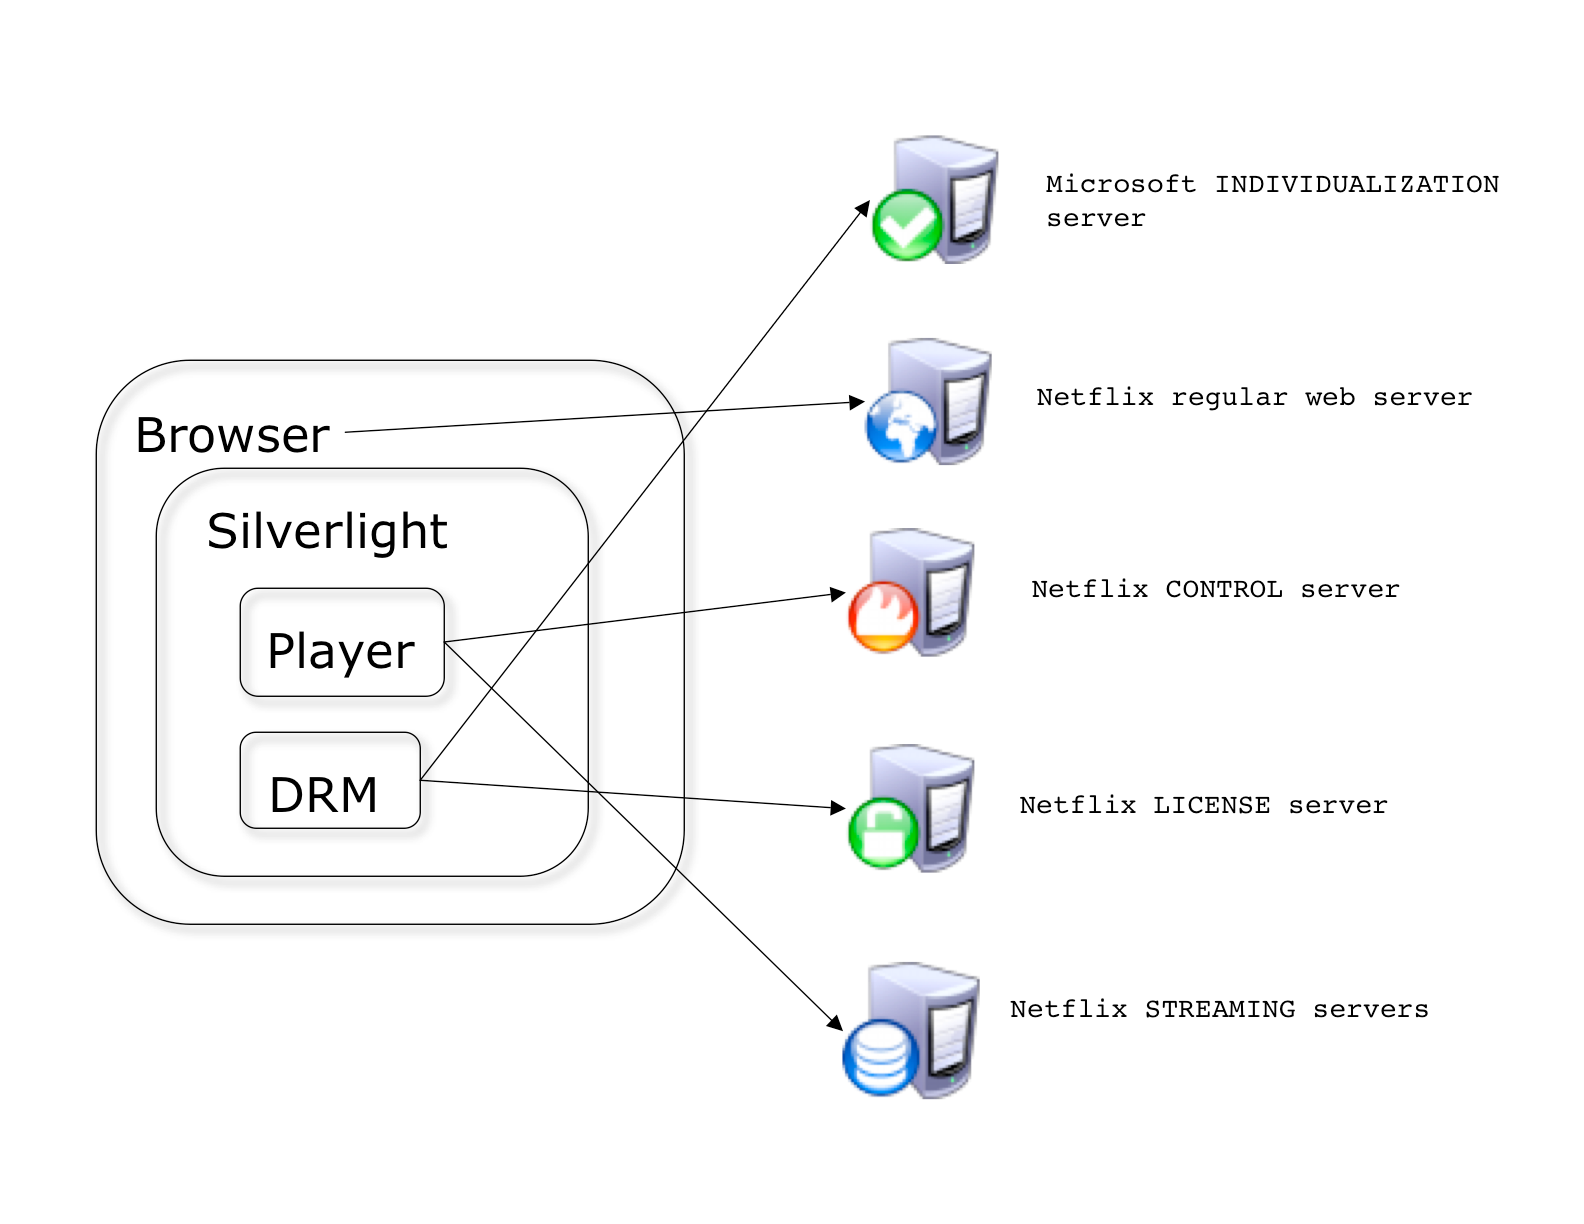
\includegraphics[width=14cm]{Figuras/autenticacao_conteudo.png} 
\label{figura:autenticacao_conteudo}
\end{figure}